\documentclass[twoside,11pt]{homework}
\usepackage{listings}
\usepackage{xcolor}
\usepackage{graphicx} 

\coursename{COMS 4771 Machine Learning (2018 Fall)} 

\studname{Jing Qian}    % YOUR NAME GOES HERE
\studmail{jq2282@columbia.edu}% YOUR UNI GOES HERE
\hwNo{2}                   % THE HOMEWORK NUMBER GOES HERE
\date{\today} % DATE GOES HERE


\begin{document}
\maketitle

%%%%%%%%%%%%%%%%%%%%%%%%%%%%%%%%%
\section*{Problem 3}
\subsection*{i)}
\color{red} (
HYY reminded, convex + convex = convex, could be used for iv prove! \\
Use GD for P5, discussed, 100,000 data points, 9000 users and 600 movies, $k \le 10$.
Since it is convex, any GD is OK.\\
draft added by Jing) \color{black} \\
The generative model for the rating of movie $j$ by user $i$ is:
%
\begin{equation}
r_{i, j} = u_i \cdot v_j + \epsilon_{i, j}
\end{equation}
%
where $\epsilon_{i, j}$ is distributed as independent zero-mean and $\sigma^2$-variance Gaussian noise.
So $r_{i, j} = N(u_i \cdot v_j, \sigma^2)$.
The parameters are  $u_i$, $v_j$ and $\sigma$ in which $u_i$ are $n \times k$ matrix, $v_j$ are $d\times k$ matrix and $\sigma$ is a real number.
So the total number of parameters is $(n+d)\times k + 1$.

%%%%%%%%%%%%%%%%%%%%%%%%%%%%%%%%%
\subsection*{ii)}
The maximum likelihood estimation of parameters are:
%
\begin{equation}
\mathrm{MLE} %&=  \mathrm{arg\ max}_{u_i \cdot v_j} \mathcal{L}(u_i \cdot v_j|r_{i,j}) \\
= \mathrm{arg\ max}_{u_i \cdot v_j} \prod_{i=1}^n \prod_{j=1}^d p(r_{i,j}|u_i \cdot v_j)
\label{mle}
\end{equation}
%
The likelihood above is the objective want to optimize (maximize).
There are no constraints other than the domain constrains: 
$u_i$ and $v_j$ are both k-dimensional vector and $r_{i, j}$ is a real number.

\subsection*{iii)}
Using the \textit{negative log likelihood} function, Eq.~\ref{mle} could be optimized as:
%
\begin{equation}
\begin{split}
\mathrm{MLE} &= \mathrm{arg\ max}_{u_i \cdot v_j} \prod_{i=1}^n \prod_{j=1}^d p(r_{i,j}|u_i \cdot v_j) \\
		      &= \mathrm{arg\ min}_{u_i \cdot v_j} \sum\limits_{i=1}^n \sum\limits_{j=1}^d - \log p(r_{i,j}|u_i \cdot v_j) \\
		      &= \mathrm{arg\ min}_{u_i \cdot v_j} \sum\limits_{i=1}^n \sum\limits_{j=1}^d (u_i \cdot v_j - r_{i, j})^2 \\
		      &= \mathrm{arg\ min}_{u_i \cdot v_j} \sum\limits_{i=1}^n \sum\limits_{j=1}^d (u_i \cdot v_j)^2 - 2r_{i, j} (u_i \cdot v_j)
\label{mle2}		      
\end{split}
\end{equation}
%
We get the optimized form above ignoring terms independent of $u_i$ and $v_j$, as discussed in Lec 5.

%%%%%%%%%%%%%%%%%%%%%%%%%%%%%%%%%
\subsection*{iv)}
Yes, the negative log-likelihood problem formulation in part (iii) is a convex optimization problem with respect to the paramter $u_i$ or $v_j$.

A problem is  a convex problem when and only when both function and constraints are convex.
As we discussed in part (ii), there is no constraint we need to worry about.
So we only need to show that the negative log-likelihood problem formulation in part (iii)  is convex with respect to the parameter $u_i$ or $v_j$.
As we could see, the formulation in part (iii) is  twice continuously differentiable. 
So if its Hessian matrix of second partial derivatives with respect to  $u_i$ (or $v_j$) is positive semidefinite, the fuction is convex and hence the optimization problem is convex.
\footnote{See the definition of convex function and Hessian matrix in wikipedia:
https://en.wikipedia.org/wiki/Convex\_function, https://en.wikipedia.org/wiki/Hessian\_matrix.}

Let's look at $u_i$ first.
Since $u_i$ and $v_j$ are both $k$-dimensional, they could be expressed as $u_i = [u_i^{(1)}, u_i^{(2)}, \cdots, u_i^{(k)}]^{\mathrm{T}}$, $v_j = [v_j^{(1)}, v_j^{(2)}, \cdots, v_j^{(k)}]^{\mathrm{T}}$.
Let $F = \sum\limits_{i=1}^n \sum\limits_{j=1}^d (u_i \cdot v_j)^2 - 2r_{i, j} (u_i \cdot v_j)$.
$\frac{\partial F}{\partial u_i} = \sum\limits_{j=1}^d 2(u_i \cdot v_j- r_{i, j})  v_j$.
%
\begin{equation}
\begin{split}
\frac{\partial^2 F}{\partial u_i ^2} &= \left [ 
						 \begin{matrix}
						 	\sum\limits_{j=1}^d 2(v_j^{(1)})^2 & \sum\limits_{j=1}^d 2v_j^{(1)}v_j^{(2)}	   \cdots \sum\limits_{j=1}^d 2v_j^{(1)}v_j^{(k)}   \\
							\sum\limits_{j=1}^d 2v_j^{(2)}v_j^{(1)} & \sum\limits_{j=1}^d 2(v_j^{(2)})^2	   \cdots \sum\limits_{j=1}^d 2v_j^{(2)}v_j^{(k)} \\
							\qquad \cdots \\
							\sum\limits_{j=1}^d 2v_j^{(k)}v_j^{(1)} & \sum\limits_{j=1}^d 2v_j^{(k)}v_j^{(2)}	   \cdots \sum\limits_{j=1}^d 2(v_j^{(k)})^2
						 \end{matrix}
						\right ] \\
					    &=\sum\limits_{j=1}^d 2\left [ 
						 \begin{matrix}
						 	 (v_j^{(1)})^2 &  v_j^{(1)}v_j^{(2)}   \cdots  v_j^{(1)}v_j^{(k)}   \\
							 v_j^{(2)}v_j^{(1)} & (v_j^{(2)})^2	   \cdots v_j^{(2)}v_j^{(k)} \\
							\qquad  \cdots \\
							v_j^{(k)}v_j^{(1)} & v_j^{(k)}v_j^{(2)}	   \cdots (v_j^{(k)})^2
						 \end{matrix}
						\right ] \\
					     &= \sum\limits_{j=1}^d 2f_j
\end{split}
\end{equation}
%
Where 
%
\begin{equation}
f_j = \left [ 
						 \begin{matrix}
						 	 (v_j^{(1)})^2 &  v_j^{(1)}v_j^{(2)}   \cdots  v_j^{(1)}v_j^{(k)}   \\
							 v_j^{(2)}v_j^{(1)} & (v_j^{(2)})^2	   \cdots v_j^{(2)}v_j^{(k)} \\
							\qquad  \cdots \\
							v_j^{(k)}v_j^{(1)} & v_j^{(k)}v_j^{(2)}	   \cdots (v_j^{(k)})^2
						 \end{matrix}
						\right ] 
\end{equation}
%
If we could prove that real matrix $f_j$ is positive semidefinite, then $\frac{\partial^2 F}{\partial u_i ^2}$, as the sum of $f_j$ is also positive semidefinite.
$v_j$ is defined as a $k$-dimensional vector and $f_j = v_j v_j^{\mathrm{T}} = <v_j, v_j>$, so $f_j$ is a Gram matrix and hence is always positive semidefinite.
\footnote{
See the definition of Gram matrix in wikipedia:
https://en.wikipedia.org/wiki/Gramian\_matrix}

In conclusion, as a Gram matrix, $f_j$ is  positive semidefinite.
The sum of $f_j$, $\frac{\partial^2 F}{\partial u_i ^2}$, which is the second partial derivatives of $F = \sum\limits_{i=1}^n \sum\limits_{j=1}^d (u_i \cdot v_j)^2 - 2r_{i, j} (u_i \cdot v_j)$ with respect to $u_i$, is also positive semidefinite.
So the function $F$ is convex and the optimization is a convex problem with respect to the parameter $u_i$.

Similarly, for parameter $v_j$, we have:
%
\begin{equation}
\begin{split}
\frac{\partial^2 F}{\partial v_j ^2} &= \left [ 
						 \begin{matrix}
						 	\sum\limits_{i=1}^n 2(u_i^{(1)})^2 & \sum\limits_{i=1}^n 2u_i^{(1)}u_i^{(2)}	   \cdots \sum\limits_{i=1}^n 2u_i^{(1)}u_i^{(k)}   \\
							\sum\limits_{i=1}^n 2u_i^{(2)}u_i^{(1)} & \sum\limits_{i=1}^n 2(u_i^{(2)})^2	   \cdots \sum\limits_{i=1}^n 2u_i^{(2)}u_i^{(k)} \\
							\qquad \cdots \\
							\sum\limits_{i=1}^n 2u_i^{(k)}u_i^{(1)} & \sum\limits_{i=1}^n 2u_i^{(k)}u_i^{(2)}	   \cdots \sum\limits_{i=1}^n 2(u_i^{(k)})^2
						 \end{matrix}
						\right ] \\
					    &=\sum\limits_{i=1}^n 2\left [ 
						 \begin{matrix}
						 	 (u_i^{(1)})^2 &  u_i^{(1)}u_i^{(2)}   \cdots  u_i^{(1)}u_i^{(k)}   \\
							 u_i^{(2)}u_i^{(1)} & (u_i^{(2)})^2	   \cdots u_i^{(2)}u_i^{(k)} \\
							\qquad  \cdots \\
							u_i^{(k)}u_i^{(1)} & u_i^{(k)}u_i^{(2)}	   \cdots (u_i^{(k)})^2
						 \end{matrix}
						\right ] \\
					     &= \sum\limits_{i=1}^n 2g_i
\end{split}
\end{equation}
%
Where 
%
\begin{equation}
g_i = \left [ 
						 \begin{matrix}
						 	 (u_i^{(1)})^2 &  u_i^{(1)}u_i^{(2)}   \cdots  u_i^{(1)}u_i^{(k)}   \\
							 u_i^{(2)}u_i^{(1)} & (u_i^{(2)})^2	   \cdots u_i^{(2)}u_i^{(k)} \\
							\qquad  \cdots \\
							u_i^{(k)}u_i^{(1)} & u_i^{(k)}u_i^{(2)}	   \cdots (u_i^{(k)})^2
						 \end{matrix}
						\right ] 
\end{equation}
%
Similar prove as before, as a Gram matrix, $g_i = u_i u_i^{\mathrm{T}} = <u_i, u_i>$ is  positive semidefinite.
The sum of $g_i$, $\frac{\partial^2 F}{\partial v_j ^2}$, which is the second partial derivatives of $F = \sum\limits_{i=1}^n \sum\limits_{j=1}^d (u_i \cdot v_j)^2 - 2r_{i, j} (u_i \cdot v_j)$ with respect to $v_j$, is also positive semidefinite.
So the function $F$ is convex and the optimization is a convex problem with respect to the parameter $v_j$.

%%%%%%%%%%%%%%%%%%%%%%%%%%%%%%%%%
\subsection*{v)}
Yes, the negative log-likelihood problem formulation (in part (iii)) is jointly convex in the parameters $u_i$ and $v_j$ simultaneously.

As discussed in part (iv), there is no constraints on the optimizing objective, we only need to prove the objective function is convex.
We could use the definition of convex function to prove it, which is:
$\beta f(x) + (1-\beta) f(x') \ge f(\beta x + (1-\beta) x')$ for $\beta \in [0, 1]$.
Here $x = u_i \cdot v_j$ and $x' = u_i' \cdot v_j'$, which are both real numbers.
$u_i$, $u_i'$, $v_j$ and $v_j'$ are $k$-dimensional vectors.
We choose two sets of parameters $(u_i, v_j)$ and $(u_i', v_j')$ to discuss the jointly convex property of the function.
Then we have:
%
\begin{equation}
\begin{split}
f(x) &=  (u_i \cdot v_j)^2 - 2r_{i, j} (u_i \cdot v_j) \\
f(x') &=  (u_i' \cdot v_j')^2 - 2r_{i, j} (u_i' \cdot v_j') \\
f(\beta x + (1-\beta) x') &= [\beta (u_i \cdot v_j) + (1-\beta) (u_i' \cdot v_j')]^2 - 2 r_{i, j}[\beta (u_i \cdot v_j) + (1-\beta) (u_i' \cdot v_j')]
\end{split}
\end{equation}
%
Then:
%
\begin{equation}
\begin{split}
&\beta f(x) + (1-\beta) f(x') - f(\beta x + (1-\beta) x') \\
=& \beta (u_i \cdot v_j)^2 - 2\beta r_{i, j} (u_i \cdot v_j) +  (1-\beta) (u_i' \cdot v_j')^2 - 2r_{i, j}(1-\beta)  (u_i' \cdot v_j') \\
&- [\beta (u_i \cdot v_j) + (1-\beta) (u_i' \cdot v_j')]^2 + 2 r_{i, j}[\beta (u_i \cdot v_j) + (1-\beta) (u_i' \cdot v_j')] \\
=& \beta (u_i \cdot v_j)^2 + (1-\beta) (u_i' \cdot v_j')^2 - [\beta (u_i \cdot v_j) + (1-\beta) (u_i' \cdot v_j')]^2 \\
=& \beta (u_i \cdot v_j)^2 + (1-\beta) (u_i' \cdot v_j')^2 - [\beta^2 (u_i \cdot v_j)^2 + (1-\beta)^2 (u_i' \cdot v_j')^2 + 2\beta (1-\beta)(u_i \cdot v_j) (u_i' \cdot v_j') ] \\
=& \beta (1-\beta) (u_i \cdot v_j)^2 + \beta (1-\beta)(u_i' \cdot v_j')^2 - 2\beta (1-\beta)(u_i \cdot v_j) (u_i' \cdot v_j') \\
=& \beta (1-\beta) (u_i \cdot v_j - u_i' \cdot v_j')^2 \\
\ge & 0 \quad (\mathrm{for} \beta \in [0, 1])
\end{split}
\end{equation}
%
In other words, $\beta f(x) + (1-\beta) f(x') \ge f(\beta x + (1-\beta) x')$ for $\beta \in [0, 1]$.
And this inequally holds for any choice of $u_i$ and $v_j$.
So the negative log-likelihood problem formulation (in part (iii)) jointly convex in the parameter $u_i$ and $v_j$ simultaneously.

%%%%%%%%%%%%%%%%%%%%%%%%%%%%%%%%%
\subsection*{vi)}
As we discussed in part (iv), the first derivative of $F = \sum\limits_{i=1}^n \sum\limits_{j=1}^d (u_i \cdot v_j)^2 - 2r_{i, j} (u_i \cdot v_j)$ with respect to $u_i$ is $\frac{\partial F}{\partial u_i} = \sum\limits_{j=1}^d 2(u_i \cdot v_j- r_{i, j})  v_j$.
Since $F$ is a convex function with respect to $u_i$, $F$ reaches minimum when $\frac{\partial F}{\partial u_i} = 0$.
In other words,
%
\begin{equation}
\sum\limits_{j=1}^d 2(u_i^* \cdot v_j- r_{i, j})  v_j = 0
\end{equation}
%
in which $u_i^*$ refers to the optimal setting of $u_i$.
If we consider $v_j$ for $j$ from 1 to $d$ as linearly independent, then we have:
%
\begin{equation}
u_i^* \cdot v_j- r_{i, j} = 0
\end{equation}
%
which holds for every $j$ value and could be used to get  $u_i^*$ if $k = d$.
If $k \neq d$, we could not get $u_i^*$ directly from the equation above.

Similarly, we could have the optimal setting of the parameter $v_j$, $v_j^*$ as following:
%
\begin{equation}
u_i \cdot v_j^j- r_{i, j} = 0
\end{equation}
%
which holds for every $i$ value and could be used to get  $v_j^*$ if $k = n$.
If $k \neq n$, we could not get $v_j^*$ directly from the equation above.

%%%%%%%%%%%%%%%%%%%%%%%%%%%%%%%%%
\subsection*{vii)}
As we discussed in part (i), we predict the rating from Gaussian distribution $r_{i, j} = N(u_i \cdot v_j, \sigma^2)$ in which $u_i$ and $v_j$ are both $k$-dimensional vectors.
If given a new/previously unseen user $\tilde{u}$ or item $\tilde{v}$, we could not give a prediction because we don't know what $\tilde{u}$ or $\tilde{v}$ is.

One way to fix it: we take $\tilde{u}$ as the mean of all known $u_i$. 
Then we could give prediction based on the estimated  $\tilde{u}$: $r_{\tilde{i}, j} = N(\tilde{u} \cdot v_j, \sigma^2) = N(\mathrm{mean}[u] \cdot v_j, \sigma^2)$.
Correspondingly, for a new/previously unseen item $\tilde{v}$, take it as the mean of all known $v_j$ and make prediction as: $r_{i, \tilde{j}} = N(u_i \cdot \tilde{v}, \sigma^2) = N(u_i \cdot \mathrm{mean}[v], \sigma^2)$.

\color{red}(other approach?) \color{black}


%%%%%%%%%%%%%%%%%%%%%%%%%%%%%%%%%
\section*{Problem 4}
\subsection*{i)}
\color{red} (
Find better solution!!!\\
draft added by Jing, need to be modified!) \color{black} \\
The mapping function is:
%
\begin{equation}  
\Phi_{\alpha, B}: x \rightarrow (1[B > \gamma > x-\alpha])_{\gamma \in \mathbb{R}}.
\end{equation}
%
For any point $x$, we could always find  an infinite dimensional weight vector $w(\gamma)$ to keep the label sign$(x)$ while doing the feature transformation. 
Due to the transformation, we have:
%
\begin{equation}
\mathrm{sign}(\int_{-\infty}^{\infty} w(\gamma) \cdot \gamma d\gamma ) = \mathrm{sign}(\int_{x - \alpha}^B w(\gamma) d\gamma)
\end{equation}
%
which means only the $w(\gamma) $ for $\gamma \in (x - \alpha, B)$ are assigned to keep the sign of $x$.

We could use induction method to show that the mapping can linearly separate any binary labeling of the $n$ points.
If $n=2$, supposing $x_1$  is positive,  $x_2$ is negative and $x_1 > x_2$.
We have:
%
\begin{equation}
\mathrm{sign}(\int_{x_1 - \alpha}^B w(\gamma) d\gamma) = 1.
\end{equation}
%
We could choose $w(\gamma) = 1$ for $\gamma \in (x_1 - \alpha, B)$.
Then
%
\begin{equation}
\begin{split}
-1 &= \mathrm{sign}(\int_{x_2 - \alpha}^B w(\gamma) d\gamma)  \\
    &= \mathrm{sign}(\int_{x_1 - \alpha}^B w(\gamma) d\gamma + \int_{x_2 - \alpha}^{x_1 - \alpha} w(\gamma) d\gamma) \\
    &= \mathrm{sign}(B - x_1 + \alpha + \int_{x_2 - \alpha}^{x_1 - \alpha} w(\gamma) d\gamma)
\end{split}
\end{equation}
%
Let $F_1 =(\int_{x_1 - \alpha}^B w(\gamma) d\gamma) = B - x_1 + \alpha $
We could choose $w(\gamma)  = \frac{-2F_1}{x_1 - x_2}$ for $\gamma \in (x_2 - \alpha, x_1 - \alpha)$.
Because  $w(\gamma) < \frac{x_1 - B- \alpha}{x_1 - x_2}$ for $\gamma \in (x_2 - \alpha, x_1 - \alpha)$, $\mathrm{sign}(\int_{x_2 - \alpha}^B w(\gamma) d\gamma) = -1$.
The transformation of $x_1$ and $x_2$ are separable.

If $x_1, \cdots, x_i$ are linearly separable by the mapping with weight vector $w(\gamma)$, the point $x_{i+1}$ has different label with $x_i$. 
Let $F_i = (\int_{x_i - \alpha}^B w(\gamma) d\gamma)$, we could have $w(\gamma)  = \frac{-2F_i}{x_i - x_{i+1}}$ for $\gamma \in (x_{i+1} - \alpha, x_i - \alpha)$.
Similarly, we have :
%
\begin{equation}
\begin{split}
\mathrm{sign} (x_{i+1}) &= \mathrm{sign}(\int_{x_{i+1} - \alpha}^B w(\gamma) d\gamma) \\
&= \mathrm{sign}(\int_{x_i - \alpha}^B w(\gamma) d\gamma + \int_{x_{i+1} - \alpha}^{x_i - \alpha} w(\gamma) d\gamma) \\
&= \mathrm{sign}(F_i - 2F_i) \\
&= - \mathrm{sign} (F_i) \\
&= - \mathrm{sign}(\int_{x_i - \alpha}^B w(\gamma) d\gamma) \\
&= - \mathrm{sign}(x_i)
\end{split}
\end{equation}
%
So $x_i$ and $x_{i+1}$ are linearly sepearable.
In conclusion, for any $n$ distinct points $x_1, \cdots, x_n \in [-B, B]$, there exists $\alpha >0 $ such that the mapping $\Phi_{\alpha, B}$ can linearly separate any binary labeling of the $n$ points. 
We only needs to assign the weight vector section by section.


\subsection*{ii)}
%
\begin{equation}
\begin{split}
\Phi_{\alpha, B} (x) \cdot \Phi_{\alpha, B} (x') &= \int_{-\infty}^{\infty} 1[B > \gamma > x-\alpha] \cdot 1[B > \gamma > x'-\alpha]\ d\gamma \\
&= \int_{\max(x - \alpha, x' - \alpha)}^B 1\ d\gamma \\
&= B - \max(x, x') + \alpha
\end{split}
\end{equation}
%

%%%%%%%%%%%%%%%%%%%%%%%%%%%%%%%%%
\section*{Problem 5}
\subsection*{ii)}
In Q3, we model the rating of movie $j$ from user $i$ as $r_{i, j} = N( u_i \cdot v_j, \sigma^2)$ which has a $u_i \cdot v_j$-mean and $\sigma^2$-variance Gaussian distribution.
Parameters $u_i,\ v_j \in \mathcal{R}^k$ are $k$-demensional vectors for $i$ from 1 to $n$ and $j$ from 1 to $d$ and $\sigma^2$ is a real number.
As suggested in Q3, parameters above could be estimated from minimize the negative log likelihood function. 
Then we have:
%
\begin{equation}
\begin{split}
\sigma^2 &= \mathrm{argmin}_{\sigma^2} \sum\limits_{i=1}^n  \sum\limits_{j=1}^d \frac{1}{2}\log \sigma^2 + \frac{(u_i \cdot v_j - r_{i, j})^2}{2\sigma^2} \\
	     &= \frac{\sum\limits_{i=1}^n  \sum\limits_{j=1}^d (u_i \cdot v_j - r_{i, j})^2}{\sum\limits_{i=1}^n  \sum\limits_{j=1}^d 1}
\end{split}
\label{sigma2}
\end{equation}
%
%\color{red}
Similar to the 1-d Gaussian distribution, we could find the optimal value for $\sigma^2$ using the stationary point.
%\color{black}

However, as we have shown in Q3 (vi), we could not get the parameters $u_i$ or $v_j$ directly from the stationary point of the negative log likelihood function.
Instead, we could use the Gradient Descent method to get to the minimum of  $F = \sum\limits_{i=1}^n \sum\limits_{j=1}^d (u_i \cdot v_j)^2 - 2r_{i, j} (u_i \cdot v_j)$
As we discussed in Q3 (iv), $F$ is convex with respect to the parameter $u_i$ or $v_j$.
Also, as in Q3 (v), $F$ is jointly convex in parameters $u_i$ and $v_j$.
Since $F$ is a convex function, the local minimum we find is in fact the global minimum.
As we discussed in Q1, different Gradient Descent methods give similar accuracy for convex functions and  converges to the minimum quickly.
So we use Stochastic Gradient Descent method for all the $u_i$ and $v_j$.

Similar to what we did in part (i), we split the whole dataset into two sets: training and testing, which has a ratio of sample sizes as 3 : 1.
In the training process, we randomly initialize $u_i$ and $v_j$ vectors and then update $u_i$ and $v_j$ using SGD: 
%
\begin{equation}
\begin{split}
u_i' &= u_i - \alpha \frac{\partial F}{\partial u_i} \\
v_j' &= v_j - \alpha \frac{\partial F}{\partial v_j}
\end{split}•
\end{equation}•
%
where the partial derivative of $F$ are:
%
\begin{equation}
\begin{split}
\frac{\partial F}{\partial u_i} &= \sum\limits_{j=1}^d 2(u_i \cdot v_j- r_{i, j})  v_j \\
\frac{\partial F}{\partial v_j} &= \sum\limits_{i=1}^n 2(u_i \cdot v_j- r_{i, j})  u_i
\end{split}•
\end{equation}•
%
We get the optimal estimation of $u_i$ and $v_j$ when $F$ reaches minimum, then get corresponding optimal $\sigma^2$ from Eq.~\ref{sigma2}.

In the testing process, we give prediction as $y_l = r_{i, j} = N( u_i \cdot v_j, \sigma^2)$ with $u_i$, $v_j$ and $\sigma^2$ from training.
Then we use the mean square error (MSE) to evaluate the performance:
%
\begin{equation}
MSE = \frac{1}{m} \sum\limits_{l=1}^m (y_l - \hat{y_l})
\end{equation}•
%
where $y_l$ is the prediction and $y_l$ is the label from testing set.


In the code for SGD method, we have three hyperparameters: the number of features $k$ in $u_i$ or $v_j$, the learning rate and the number of iterations.

First, let's look at the number of features. 
Since  there are about 9000 movies and about 600 users, using the conclusion from Q3.(i), we have $(n+d)k+1 \approx 9600 k$ variables.
The datafile contains around 100, 000 movie ratings.
To avoid redundant features, we should have an upper bound of $k$ that ensures $9600 k < 100, 000$.
In other words, $k < 10$.
Considering the training sample is about 3/4 of all the movie ratings, which is about 75, 000 records, the actual $k$ might be even smaller.
On the other hand, $k$ should not be too small because the model would be too simplified and the error would be large.
So we fixed $\alpha = 0.01$ and 10 iterations and tested $k = [1,3,5,7,9]$.
In Fig.~\ref{Fk}, we show the training MSE and testing MSE as the function of $k$.
From this plot, we could see that the training MSE is larger than testing MSE with all $k$ values.
The MSE decreases with the increasing $k$ while the MSE lines are quite flat when $k$ increases from 7 to 9.
For the running efficiency and based on our previous discussion, we choose $k = 7$.

%
%%%%%%%%%%%%%%%%%%% Fig. 1 %%%%%%%%%%%%%%%%%%%%%%%%%%%%%%
\begin{figure}[ht]
\centering
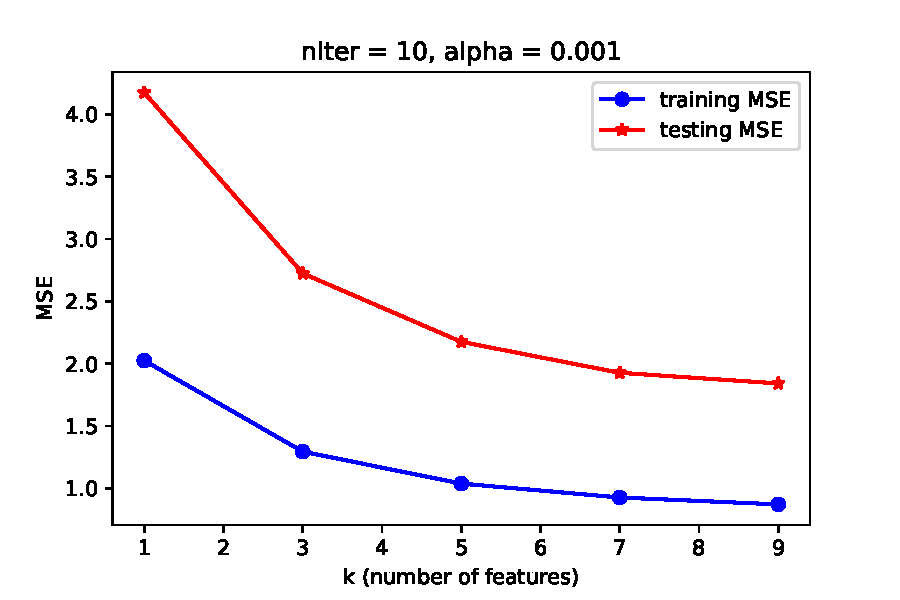
\includegraphics[]{kTest.pdf}
\caption{Performance of SGD method as a function of $k$.}
\label{Fk}
\end{figure}
%%%%%%%%%%%%%%%%%%%%%%%%%%%%%%%%%%%%%%%%%%%%%%%%%%%%%
%
%#k = [1, 3, 5, 7]
%[iiter, ik, ialpha, sigma2, fTest]
%[[10, 1, 0.001, 2.0253293168660527, 4.1757134175918411], 
%[10, 3, 0.001, 1.2944756888765558, 2.7249311933214191], 
%[10, 5, 0.001, 1.0377627835887968, 2.1754462643143611], 
%[10, 7, 0.001, 0.92637840983188213, 1.9270066912573265], 
%[10, 9, 0.001, 0.87085992982109028, 1.8417170263856335]]

Then, the learning rate.
As we discussed in Q1, the learning rate should not be too small, or in limited iterations, it may not descent enough and not reach minimum.
On the other hand, it should not be too big, or it may skip the minimum, jumping back and forth.
So we fixed $k = 7$ and 10 iterations and tested $\alpha = [0.0005, 0.001, 0.005, 0.01, 0.03]$.
%
%%%%%%%%%%%%%%%%%%% Fig. 2 %%%%%%%%%%%%%%%%%%%%%%%%%%%%%%
\begin{figure}[ht]
\centering
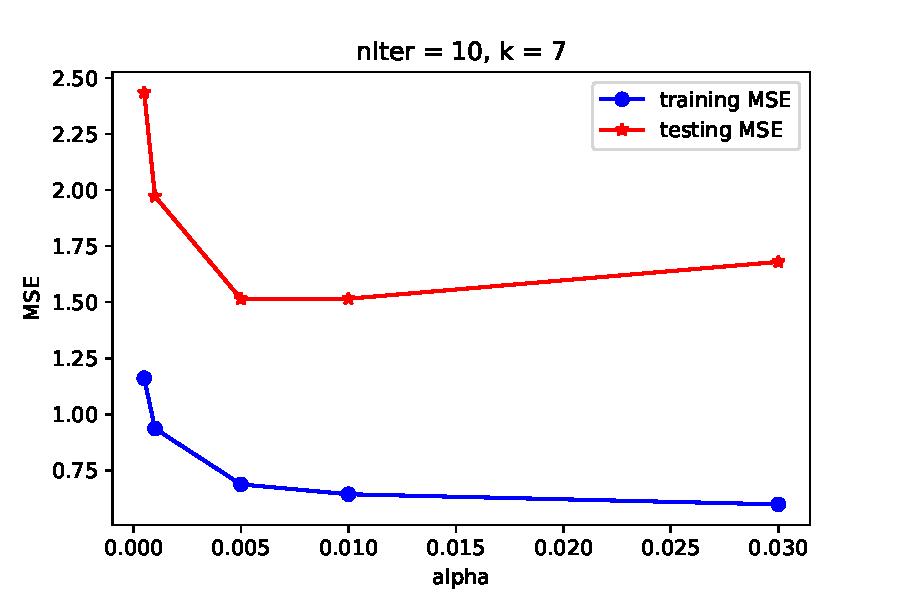
\includegraphics[]{alphaTest.pdf}
\caption{Performance of SGD method as a function of $\alpha$.}
\label{Falpha}
\end{figure}
%%%%%%%%%%%%%%%%%%%%%%%%%%%%%%%%%%%%%%%%%%%%%%%%%%%%%
%
In Fig.~\ref{Falpha}, we show the training MSE and testing MSE as the function of $\alpha$.
From this plot, we could see that the training MSE is larger than testing MSE with all $\alpha$ values.
The training MSE decreases with the increasing $\alpha$.
When $\alpha$ increases from 0.0005 to 0.005, the training MSE drops significantly but when  $\alpha$ increases tremendously increases from 0.005 to 0.03, the training MSE is quite flat.
The testing MSE shows similar trend while has a slight increasement with $\alpha$ increasing from 0.005 to 0.03.
So we choose $\alpha = 0.005$.
%%%%%%%%%%%%%
%niter = [10]
%    k = [7]
%    alpha = [0.0005, 0.001, 0.005, 0.01]
%[10, 7, 0.0005, 1.1610642484652545, 2.4342780417296268], 
%[10, 7, 0.001, 0.93644897700535501, 1.9720280374481791], 
%[10, 7, 0.005, 0.68747190800946478, 1.5144081714147259], 
%[10, 7, 0.01, 0.64360067986615332, 1.5152522760919713],
%[10, 7, 0.03, 0.598187688024, 1.67944232436]
%#break at 0.06

Finally, the number of iterations. 
Ideally, we would want to stop the gradient descent when $F$ reaches minimum, which means the partial derivatives are zero. 
But in reality, it takes a lot of running time which usually seems unnecessary.
We don't need $F$ to be minimum, instead we want it to be small enough.
So people commonly set a maximum to limit the iteration number. 
Generally speaking, if we choose proper $k$ and proper $alpha$, the MSE would decrease with the increasement of iteration number, as shown in Fig.~\ref{FnIter}.
We fixed $k=7$ and $\alpha = 0.005$ and tested number of iterations = $[10, 50, 100]$.
%
%%%%%%%%%%%%%%%%%%% Fig. 3 %%%%%%%%%%%%%%%%%%%%%%%%%%%%%%
\begin{figure}[ht]
\centering
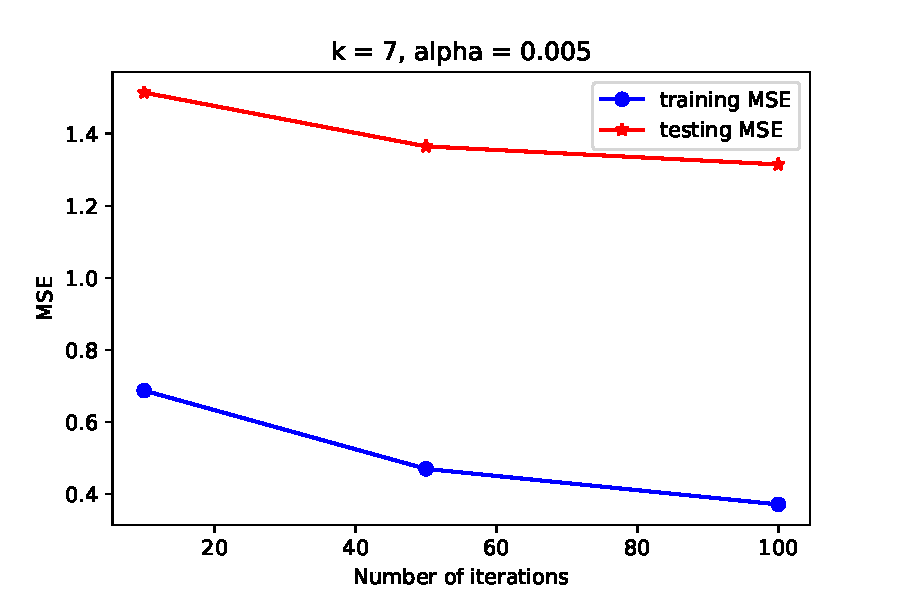
\includegraphics[]{nIterTest.pdf}
\caption{Performance of SGD method as a function of iteration number.}
\label{FnIter}
\end{figure}
%%%%%%%%%%%%%%%%%%%%%%%%%%%%%%%%%%%%%%%%%%%%%%%%%%%%%
%
%[[10, 7, 0.005, 0.68747190800946478, 1.5144081714147259], 
%[50, 7, 0.005, 0.470210070906, 1.36518009696],
%[100, 7, 0.005, 0.371584932337, 1.31504151988]]

In conclusion, we implement the model in Q3 with $u_i$ and $v_j$ optimized with Stochastic Gradient Descent method (and $\sigma^2$ based on $u_i$ and $v_j$).
We choose $k = 7, \alpha = 0.005$ and 100 iterations for 75627 training ratings and 25209 testing ratings.
Because of the computation resouce limit, we only seperated datasets into training and testing sets and tried several parameters.
A better way to do it is to use $k$-fold cross validation to choose the optimal combination of parameters.
Also, the parameters should be combined to do parameter seach, instead of what we do here, which is fixing 2 parameters and discuss the rest one parameter.

\subsection*{iii)}
 
\end{document} 
